% Copyright (C) 2014-2016 by Thomas Auzinger <thomas@auzinger.name>

\documentclass[draft,final]{vutinfth} % Remove option 'final' to obtain debug information.
%\documentclass[draft,final]{vutinfth} % Remove option 'final' to obtain debug information.

% Load packages to allow in- and output of non-ASCII characters.
\usepackage{lmodern}        % Use an extension of the original Computer Modern font to minimize the use of bitmapped letters.
\usepackage[T1]{fontenc}    % Determines font encoding of the output. Font packages have to be included before this line.
\usepackage[utf8]{inputenc} % Determines encoding of the input. All input files have to use UTF8 encoding.

% Extended LaTeX functionality is enables by including packages with \usepackage{...}.
\usepackage{amsmath}    % Extended typesetting of mathematical expression.
\usepackage{amssymb}    % Provides a multitude of mathematical symbols.
\usepackage{mathtools}  % Further extensions of mathematical typesetting.
\usepackage{microtype}  % Small-scale typographic enhancements.
\usepackage[inline]{enumitem} % User control over the layout of lists (itemize, enumerate, description).
\usepackage{multirow}   % Allows table elements to span several rows.
\usepackage{booktabs}   % Improves the typesettings of tables.
\usepackage{subcaption} % Allows the use of subfigures and enables their referencing.
\usepackage[labelfont=bf]{caption}
\usepackage[ruled,linesnumbered,algochapter]{algorithm2e} % Enables the writing of pseudo code.
\usepackage[usenames,dvipsnames,table]{xcolor} % Allows the definition and use of colors. This package has to be included before tikz.
\usepackage{nag}       % Issues warnings when best practices in writing LaTeX documents are violated.
\usepackage{todonotes} % Provides tooltip-like todo notes.
\usepackage{hyperref}  % Enables cross linking in the electronic document version. This package has to be included second to last.
\usepackage[acronym,toc]{glossaries} % Enables the generation of glossaries and lists fo acronyms. This package has to be included last.

\usepackage{graphicx,rotating}
\usepackage{csquotes}

% Define convenience functions to use the author name and the thesis title in the PDF document properties.
\newcommand{\authorname}{Lukas Baronyai} % The author name without titles.
\newcommand{\thesistitle}{An Evaluation Framework for LD Solutions} % The title of the thesis. The English version should be used, if it exists.
\newcommand{\thesissubtitle}{a case study at TU Wien} % The subtitle of the thesis. The English version should be used, if it exists.

% Set PDF document properties
\hypersetup{
    pdfpagelayout   = TwoPageRight,           % How the document is shown in PDF viewers (optional).
    linkbordercolor = {Melon},                % The color of the borders of boxes around crosslinks (optional).
    pdfauthor       = {\authorname},          % The author's name in the document properties (optional).
    pdftitle        = {\thesistitle},         % The document's title in the document properties (optional).
    pdfsubject      = {An evaluation framework for LD Solutions},              % The document's subject in the document properties (optional).
    pdfkeywords     = {LD, linked data, linked open data, comparison, framework, LDIF, Apache, Jena, Euclid, LUCERO, Linked Data book, D2RQ, Information Workbench, Eclipse, RDF4J} % The document's keywords in the document properties (optional).
}

\setpnumwidth{2.5em}        % Avoid overfull hboxes in the table of contents (see memoir manual).
\setsecnumdepth{subsection} % Enumerate subsections.

\nonzeroparskip             % Create space between paragraphs (optional).
\setlength{\parindent}{0pt} % Remove paragraph identation (optional).

%\makeindex      % Use an optional index.
%\makeglossaries % Use an optional glossary.
%\glstocfalse   % Remove the glossaries from the table of contents.

% Set persons with 4 arguments:
%  {title before name}{name}{title after name}{gender}
%  where both titles are optional (i.e. can be given as empty brackets {}).
\setauthor{}{\authorname}{}{male}
\setadvisor{Prof. Dr.}{Stefan Biffl}{}{male}

% For bachelor and master theses:
\setfirstassistant{MSc., PhD}{Marta Sabou}{}{female}

% Required data.
\setaddress{Huttengasse 51/10, 1160 Wien}
\setregnumber{01326526}
\setdate{\the\day}{\the\month}{\the\year} % Set date with 3 arguments: {day}{month}{year}.
\settitle{\thesistitle}{\thesistitle} % Sets English and German version of the title (both can be English or German).
\setsubtitle{\thesissubtitle}{\thesissubtitle} % Sets English and German version of the subtitle (both can be English or German).

% Select the thesis type: bachelor / master / doctor / phd-school.
% Bachelor:
\setthesis{bachelor}

% For bachelor and master:
\setcurriculum{Software and Information Engineering}{Software und Information Engineering} % Sets the English and German name of the curriculum.

\usepackage[backend=bibtex,bibencoding=ascii, natbib=true, defernumbers=true, style=ieee]{biblatex}
\addbibresource{bibliography.bib}

\begin{document}

\frontmatter % Switches to roman numbering.
% The structure of the thesis has to conform to
%  http://www.informatik.tuwien.ac.at/dekanat

\addtitlepage{naustrian} % German title page (not for dissertations at the PhD School).
\addtitlepage{english} % English title page.
\addstatementpage

%%%%%%%%%%%%%%%%%%%%%%%%%%%%%%%%%%%%%%%%%%%%%%%%%%%%%%%%%%%%%%

%\begin{acknowledgements*}
\todo{Enter your text here.}
\end{acknowledgements*}
\begin{abstract}
\todo{Enter your text here.}
\end{abstract}

%%%%%%%%%%%%%%%%%%%%%%%%%%%%%%%%%%%%%%%%%%%%%%%%%%%%%%%%%%%%%%

% Select the language of the thesis, e.g., english or naustrian.
\selectlanguage{english}

% Add a table of contents (toc).
\setcounter{tocdepth}{2}
\tableofcontents % Starred version, i.e., \tableofcontents*, removes the self-entry.

% Switch to arabic numbering and start the enumeration of chapters in the table of content.
\mainmatter

%%%%%%%%%%%%%%%%%%%%%%%%%%%%%%%%%%%%%%%%%%%%%%%%%%%%%%%%%%%%%%

%some general acronyms
\newacronym{ld}{LD}{Linked Data}
\newacronym{od}{OD}{Open Data}
\newacronym{lod}{LOD}{Linked Open Data}

%%%%%%%%%%%%%%%%%%%%%%%%%%%%%%%%%%%%%%%%%%%%%%%%%%%%%%%%%%%%%%

\chapter{Introduction}

The Semantic Web is getting more and more popular and with it the need for ways to publish Linked (Open) Data. In order to cover these needs, a lot of different tools, frameworks and solutions came up, some covering the whole process of publishing L(O)D, others covering only steps in the process of it. These led to a vast diversity but also a big number of options. In order to develop a LOD project, the responsible stakeholders now have to choose among these many options.

\section{Research Question}

Aim of this paper is to compare existing and common LOD solutions to give responsible stakeholders at TU Wien a decision guidance for choosing one. The concrete research question is as following:

\textbf{RQ:} \textit{How do common LOD solutions~\footnotemark compare against each?}
\begin{enumerate}
\item \textbf{RQ1:} What are existing LOD solutions?
\item \textbf{RQ2:} What are criteria to compare solutions?
\item \textbf{RQ3:} How do they compare against each other?
\item \textbf{RQ4:} What can be a solution for TU Wien?
\end{enumerate}

The conducted work is a follow-up work of a previous study (see ~\cite{baronyai_publishing_2016}) done by the author and will build up on it.

\footnotetext{\textbf{Note}: The term \textit{solutions} is used here on purpose to abstract terms like \textit{framework}, \textit{tool} or \textit{all-in-one solution}. Using only the term \textit{framework} would lead to problems and cut out other options. For a more detailed discussion see section~\ref{def:framework}}.

\section{Methodology}

The work was done as a literature study. First a discussion of the term "framework" was done in order to achieve the research question. Then a range of existing L(O)D projects and application was investigated, to extract used technologies from them. From this, candidates were retrieved and classified. After excluding and filtering some of the candidates, they were compared in four criteria groups: Criteria from the above mentioned study, usability, data formats and the Linked Data Publishing Checklist.

\section{Structure of this Paper}
This paper starts with a state of the art section in which similar comparision will be described. The next chapter~\ref{chap:methodology} is the definition of the used methodology, where a discussion of the term "framework" will be done for this paper (section~\ref{def:framework}), the process of the literature study (section~\ref{meth_study}) and the classification (section~\ref{classification}) system will be defined.

In chapter~\ref{overview} the found solution will be reviewed and described as well as the excluded candidates (section~\ref{excluded}). In chapter~\ref{criteria} the criteria as well as their according scala will be defined. The final comparison will be done in chapter~\ref{comparison}, the summary of it can be found in section~\ref{comp_summary}.

The last research question, RQ4, will be answered in chapter~\ref{ch:tuwien}, investigating, which of the proposed solutions may be suitable for which situation at TU Wien.

The last chapter, \ref{ch:summary}, describes the overall summary and future work.
\chapter{State Of The Art}

\chapter{Methodology (RQ1)}\label{chap:methodology}
\section{About The Difficulty Of Comparing Solutions}\label{def:framework}

One could expect, that this thesis may compare "frameworks". But there comes problems with this term. What actually is a "framework"? Is the term well-defined enough to clearly refer to a solution?

\subsection{The Term "Framework"}

In order to use the term a first step must be to define \emph{what} a framework actually is, since it is a very generic term. One way to define it could be the definition by Roberts and Johnson,~\cite{roberts1996evolving}:

\begin{quotation}
Frameworks are reusable designs of all part of a software described by a set of abstract classes and the way instances of those collaborate
\end{quotation}

Another way could be the explanation by Riehle in his PhD thesis,~\cite{riehle2000framework}:

\begin{quotation}
Frameworks model a specific domain or an important aspect thereof. They represent the domain as an abstract design, consisting of abstract classes (or interfaces). The abstract design is more than a set of classes, because it defines how instances of the classes are allowed to collaborate with each other at runtime. Effectively, it acts as a skeleton, or a scaffolding, that determines how framework objects relate to each other.

A framework comes with reusable implementations in the form of abstract and concrete class implementations. Abstract implementations are abstract classes that implement parts of a framework abstraction (as expressed by an abstract class or interface), but leave crucial implementation decisions to subclasses. [...]
\end{quotation}

Both of them refer frameworks as tools for coding, used when writing own applications. One of the most classical examples might be the Spring Framework in the Java world. In the mentioned projects, Apache Jena and RDF4J mostly apply on this definition.

But the problem is here, that the term is not always used and understand in this way, LDIF and the Silk frameworks define themselves as such, but providing in facts a set of tools without necessarily needing coding to work with them (except configuration files). Others may see tools like the Information Workbench or D2RQ as a framework for publishing.

On a higher level, the architectures proposed in section~\ref{arch_frameworks} might be seen as a high-level or meta-framework. And since the proposed tools in the other sections (partially) are using these architectures, one could argue, that they therefore are also frameworks.

It can be seen, that is actually problematic to use this term in the context of this thesis since it is too broad and not well-defined. In order to solve this issue, the term "solution" will be used to abstract the term and referring either to "tool", "framework" or "all-in-one solution".

\subsection{Defining The Limits}

Next to the general problem about the term "framework", another problem is to set the borders of the examine topic. As mentioned in the introduction this thesis aims to compare LD solutions, the goal is to cover the whole process of publishing Linked Data, from the bottom persistence layer of accessing existing data, transforming data formats (e.g. relational to RDF), over cleaning and interlinking the data, over storing them in a triple store, up to making them available over an interface like SPARQL.

But there are not many tools/frameworks covering the whole process and supporting different data formats (e.g. relational data and CSV) at the same time. There are some tools like D2RQ only focusing on specific data formats, but providing the full stack, some tools like LDIF only focusing on a specific part of the process, without e.g. providing capabilities for SPARQL endpoints.

The best way is maybe using a stack of different tools to cover the whole workflow, combining them like Silk is integrated in LDIF. Or using the generic architecture, coding an own application and using partially the proposed tools.

But covering different areas, it is difficult to actually compare them. How to compare a persistence framework with a GUI framework? In order to handle this problem, a classification system will be introduced in section~\ref{classification} and the criteria introduced in section~\ref{criteria} will take this difficulty into account.

\section{Methodology Of The Literature Study}\label{meth_study}
In order to answer RQ1, a literature study was conducted, but since the scope is difficult to define as described in section~\ref{def:framework}, it was not a pure study. As the aim of this thesis is to compare \textit{common} frameworks and \textit{best practices}, it would be not sufficient to review every possible paper about a LD framework or tool, therefore another approach was chosen: deriving candidates from projects. In order to do that, the following process was used:

\begin{enumerate}
\item Identify \& find a LD application/project, ignoring the success of it
\item Find public documentation and/or scientific work of it
\item Analyse used technology, add as candidate if appropriate and if not disadvised
\item Classify candidates (see~\ref{classification})
\item Analyse reference work for possible input for 1.)
\item Analyse reference work of tool/framework at its documentation
\end{enumerate}

Using this approach led to a variety of candidates, which will be listed in section~\ref{overview}. The candidates from section~\ref{excluded} were mostly excluded because of step 2.), which ensured a better base for the following comparison.

\section{A Classification System}\label{classification}

\begin{table}[htb]
\centering
\begin{tabular}{|l|l|}
\hline
\textbf{Class}              & \textbf{Detail}                                                                                                                                                                                                                        \\ \hline
\textbf{Architecture}       & \begin{tabular}[c]{@{}l@{}}A general architecture without concrete technology. \\ A solution of this class can be used in combination \\ of any other class.\end{tabular}                                                        \\ \hline
\textbf{Full-Stack}         & \begin{tabular}[c]{@{}l@{}}A solution which covers the whole stack and \\ therefore does not need another component. \\ An "All-In-One" Solution\end{tabular}                                                                    \\ \hline
\textbf{Presentation layer} & \begin{tabular}[c]{@{}l@{}}A solution which only covers the presentation or \\ UI layer and therefore depends on other component.  \\ Managing how LD can be accessed from outside \\ and how the data are exposed.\end{tabular} \\ \hline
\textbf{Business Layer}     & \begin{tabular}[c]{@{}l@{}}A solution which only covers the business layer \\ and therefore depends on other components. \\ Managing how LD are processed.\end{tabular}                                                          \\ \hline
\textbf{Data Access Layer}  & \begin{tabular}[c]{@{}l@{}}A solution which only covers the data access layer \\ and therefore depends on other components. \\ Managing how LD are stored and accessed \\ by the application.\end{tabular}                          \\ \hline
\end{tabular}
\centering
\caption{Overview of the Classification}
\label{the_label}
\end{table}

Resulting from~\ref{def:framework} different classifications were introduced to find classification-based criteria and to balance out the vast variation of the results. The classifications can be seen in table~\ref{the_label}.

The Classifications are based on the idea, that a majority of applications are using in one way or another a variation or parts of the three layer architecture style, with components responsible for either UI, Business or Data Access. This does \textit{not} necessarily mean, that they use the full concepts of this architecture or even implementing this style. It is only assumed that a component have a responsibility mappable to one of the layers. Accordingly it is assumed, that a solution can be associated with one of these responsibilities.

It is arguable, if the differentiation between "Full-Stack" and labeling a solution with the three layer class is necessary. The additional "Full-Stack" class was added to emphasize the "All-In-One" approach of such a solution, meaning that all components are provided, no further components are need. This also means, that the included components of the different responsibilities are either harmonized to each other or do not differentiate between these responsibilities. On the other side labeling a tool with the three layer classes, does not implicit this and can also mean, that the support of each of this layer can be optional.
\chapter{Overview of solutions}\label{overview}
In order to compare frameworks an understanding of existing frameworks is necessary. This section will look at existing frameworks, what kind of frameworks they are, which of them can be used for this paper and which must be excluded. Furthermore, this section aims to understand how frameworks look like and will examine the architecture of them.

\section{Architectures Of Frameworks}\label{arch_frameworks}
In this subsection the paper will look into three proposed models how frameworks (and/or implemented LD-applications) should look like. There are many other existing architectures and ongoing projects exposing data as Linked (Open) Data, this paper will use the following as representation of them.

\newacronym{euclid}{EUCLID}{EdUcational Curriculum for the usage of Linked Data}
\subsection{Euclid Project}\index{Architectures!Euclid Project}

\begin{figure}[h]
	\centering

\includegraphics[width=0.5\textwidth]{img/euclid_logo.png}
\end{figure}

\begin{figure}[htbp]
	\centering
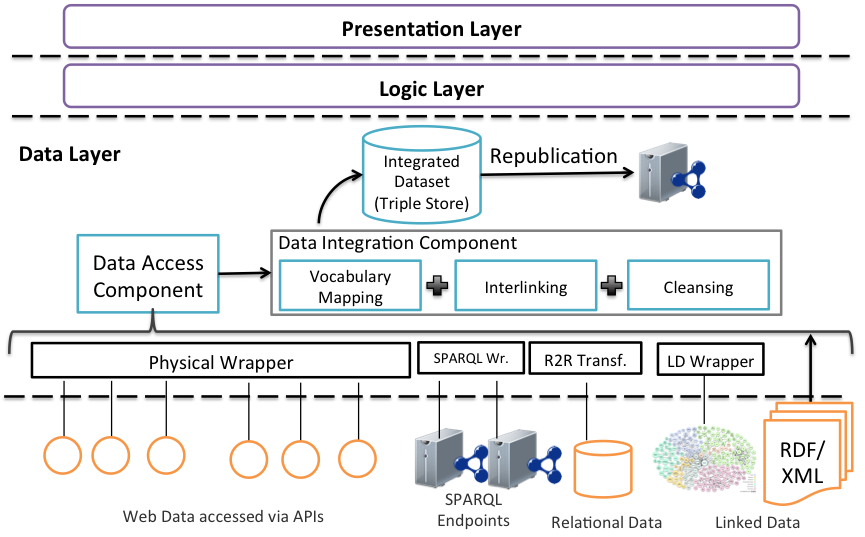
\includegraphics[width=1\textwidth]{img/euclid_architecture.png}
	\caption{General EUCLID architecture}
	\label{euclid_architecture}
\end{figure}

The EUCLID project~\footnote{~\cite{euclid:home}}(EdUcational Curriculum for the usage of Linked Data) was founded under the \emph{Seventh Framework Programme of Research and Technological Development}, a funding program of the European Union/European Commission for 2007-2013~\footnote{~\cite{eu:fp7}}\footnote{EUCLID in the CORDIS database: \url{http://cordis.europa.eu/project/rcn/103709_en.html}}.

Aim of the project was (and still is) to gather existing knowledge and expertise of \emph{"researchers, technology enthusiasts and early adopters in various European Member States"} and provide that accumulated as educational resources to enable the  full benefit of L(O)D for European businesses. The project built upon a consortium experienced in \emph{"over 20 LD projects with over 40 companies and public offices in more than 10 countries"}~\cite{euclid:about}

The outcome of this project is a a range of learning materials, fragmented into modules, and eLearning distribution channels. Overall there are six modules:

\begin{enumerate}
	\item \textbf{Introduction and Application Scenarios}
	The introduction provides the knowledge to understand, \emph{what} Linked Data are, the main principles, the standards and the required technologies. Further, an overview how to publish and to consume the data is given.
	\item \textbf{Querying Linked Data}
	This chapter mainly describes SPARQL and how to use it for querying and updating.
	\item \textbf{Providing Linked Data}
	This module deals with the production and exposure of Linked data, using the tools as R2RML (for relational databases), Open Refine (for spreadsheets), GATECloud (for natural language) and Silk (for interlinkage between datasets, see section~\ref{silk} for details about this tool)
	\item \textbf{Interaction with Linked Data}
	The projects describes in this chapter, how to explore Linked Data, using visualization tools, semantic browsers and applications, introducing search options like faceted search, concept-based search and hybrid search.
	\item \textbf{Creating Linked Data Applications}
	This module describes how to build a Linked Data Application, which technologies to use and how to integrate common Web APIs.
	\item \textbf{Scaling up}
	Finally this chapter examines the main issues of scalability regarding Linked Open Data and describes the relationship to Big Data.
\end{enumerate}

For this paper module 3 and 5~\footnote{~\cite{euclid:chap5}} are the most interesting. Module 3 describes some useful technologies for various steps on the way of exposing L(O)D, but module 5 introduce a high level architecture and some patterns, how a L(O)D application might look like (see ~\cite{euclid:chap5} for details). In detail, they provide a three-tier architecture (see figure~\ref{euclid_architecture} and three architecture patterns.

The architecture is very generic and consists of the classic three tiers: presentation, logic and data, each independent to the overlaying tier. Since the presentation and logic layer does not concern the actual publishing of the data, the data layer is the interesting one here. The layer consists of the \emph{Data Access Component}, which represents the access to different data types like relational data or other Web APIs and transforms the data to RDF, the \emph{Data Integration Component}, which does the vocabulary mapping and interlinking for the cleansing in order to e.g. identify and fix ambiguities in resource names, and finally the \emph{Triple Store}, holding the integrated dataset for exposing it to the web.

The mentioned patterns to use for implementations are:

\begin{itemize}
\item \textbf{Crawling pattern}
Used for loading the data in advance and storing them in a triple store, increasing the efficiency of data access. In exchange, the data might not be up to date when accessed
\item \textbf{On-The-Fly Dereferencing Pattern}
Meaning that the URIs are dereferenced when the application need to access the data. This pattern provides up to date data but for the cost of performance when dereference many URIs.
\item \textbf{(Federated) Query Pattern}
Describing the use of complex queries on a fix set of data sources, enabling to work with current data directly retrieved from the sources. The pattern offers an access up-to-date data with adequate response time in specific situations but for the cost of the complex problem to find optimal queries.
\end{itemize}

\newacronym{lucero}{LUCERO}{Linking University Content for Education and Research Online}
\subsection{LUCERO}\index{Architectures!LUCERO}

%\begin{figure}[htbp]
%	\centering
%
\includegraphics[width=0.15\textwidth]{img/lucero_logo.png}
%\end{figure}

\begin{figure}[htbp]
	\centering
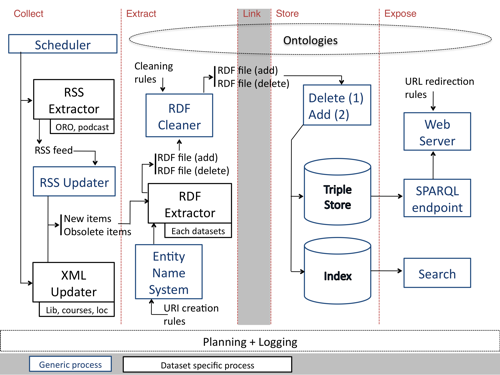
\includegraphics[width=\textwidth]{img/lucero_architecture.png}
	\caption{LUCERO work flow \& architecture}
	\label{lucero_architecture}
\end{figure}

The LUCERO project ("Linking University Content for Education and Research Online")~\footnote{The code is available in the Google Code Archive: \url{https://code.google.com/archive/p/luceroproject/wikis/StepByStepDocumentation.wiki}} was a project at the Open University, aiming to \emph{"scope, prototype, pilot and evaluate reusable, cost-effective solutions relying on the linked dataprinciples and technologies for exposing and connecting educational and research content"}. It was founded for one year by the JISC Information Environment 2011 Programme under the call Deposit of research outputs and Exposing digital content for education and research.~\cite{lucero:about}

The projects connected with other organizations through LinkedUniversities.org~\footnote{\url{http://linkeduniversities.org/}} to gather common issues and practices. The outcome was the first university linked data platform,~\url{http://data.open.ac.uk/}, with a lot of impact on The Open University and the education community.

Looking at the architecture in figure~\ref{lucero_architecture} comparing to the Euclid architecture seen in the previous section, there are quite a lot of similarities. Both have components for accessing different kinds of data, here called \emph{Extractors}, for cleaning the data, here called \emph{Cleaner}, and a Triple Store, holding the data available. The lanes "Collect", "Extract", "Link" and "Store" can be seen as the data layer from the classic three-tier architecture, the "Expose" lane as the logic and presentation layer. 

Both using the crawling pattern to extract, map and store the data in a Linked Data format instead of transforming them for every request.

\subsubsection{TABLOID}\index{Tools!TABLOID}
One of the outcomes next to the LOD application itself was the Tabloid ("Toolkit ABout Linked Open Institutional Data"), \emph{"a toolkit intended to help institutions and developers to both publish and consume linked data"}. It contains work-flows, documentations, examples and tools~\cite{lucero:tabloid} trying to address different roles such as managers, developers and users. Tabloid try to help people to understand LD, what can be done with it and give advice on a technical perspective, how to publish and consume LD, providing at the same time a detailed and generic way.

\subsection{Linked Data book}\index{Architectures!Linked Data Book}

\begin{figure}[htbp]
	\centering
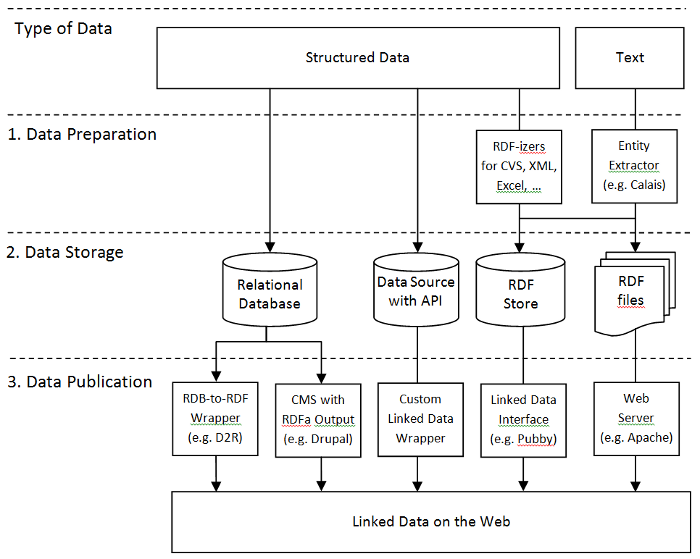
\includegraphics[width=\textwidth]{img/ld_architecture.png}
	\caption{Linked Data Publishing Options and Workflows according to the LD book}
	\label{ld_architecture}
\end{figure}

Another big effort ampng many others of describing LD in general, how to publish and consume them and how to implement applications was done by the book "Linked Data: Evolving the Web into a Global Data Space" by Heath and Bizer~\cite{heath2011linked}, which received a lot of attention.

The book aims in general to give a basic understanding of LD and describing publication and consumption of LD. They providing advices and best practices, including architectures approaches, identifying the right set of URIs and vocabulary and much more. They also described an architecture, to be seen in figure~\ref{ld_architecture}

Next to patterns they also provide a general workflow for LD publishing, see figure~\ref{ld_architecture}. But comparing to the introduced architectures in the previous sections, the workflow has a different approach: instead of holding the data in a Triple Store, the workflow access and transforms the raw data on-the-fly for every request.

Next to this workflow, the book also provides various "recipes" for publishing LD and one of them is also to hold the data in a triple store as shown by Euclid and LUCERO. Furthermore the book provides a guide for the D2R-Server, which will be described in section~\ref{d2rq}.

\newpage
\section{Frameworks}

\subsection{D2RQ Platform}\label{d2rq}\index{Framework!D2RQ Platform}

\begin{figure}[htbp]
	\centering
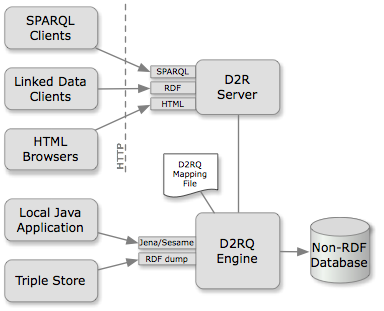
\includegraphics[width=0.8\textwidth]{img/d2rq_architecture.png}
	\caption{D2R Server architecture}
	\label{d2rq_architecture}
\end{figure}

\begin{verse}
\textbf{NOTE:} The last update on the D2RQ platform was in 2012 (version 0.8.1) and on the D2R Server in 2009 (version 0.7)
\end{verse}

The D2RQ platform~\footnote{\url{http://d2rq.org}} was introduced by the Free University of Berlin and provides a database-to-RDF mapping. It is licensed under the terms of the GNU General Public License. 

To map a relational database the platform provides a declarative mapping language, expressed in RDF, which is then be used to provide access to the database in the following, read-only, ways:~\cite{d2rq:w3c}

\begin{itemize}
\item \textbf{RDF dumps}
\item \textbf{RDF APIs}
\item \textbf{SPARQL endpoint} (D2R Server)
\item \textbf{Linked Data}
\item \textbf{HTML view} (D2R Server)
\end{itemize}

For an overview of the framework structure see figure~\ref{d2rq_architecture}.

\subsubsection{D2R Server}\index{Framework!D2RQ Platform!D2R Server}
Part of the platform is the D2R Server~\footnote{\url{http://d2rq.org/d2r-server}}, which provides the public access to the platform over SPARQL and HTML, publishing it to the semantic web. More concrete, the server provides a dereferencing interface, for HTTP request dereferencing, and a SPARQL interface. 

The server uses the mentioned \textbf{On-The-Fly Dereferencing Pattern} and does not provide a triple store, therefore it may be not has as good performance than tools with a triple store, although the team made a great effort to improve it.

Part of the server is also a tool which generates automatically a corresponding mapping and RDF vocabulary for an existing table structure, using table names as class names and column names as property names. The generated mapping file can then be customised.~\cite{bizer2006d2r}

The following applications are examples using D2R-Server:

\begin{itemize}
\item DBLP Bibliography (University of Hannover)~\footnote{\url{http://dblp.uni-trier.de/}}
\item DBtune (University of London)~\footnote{\url{http://dbtune.org/}}
\item Database of the Nobel Prize~\footnote{\url{http://data.nobelprize.org/}}
\end{itemize}

\subsection{Information Workbench}\index{Framework!Information Workbench}

\begin{figure}[htbp]
	\centering
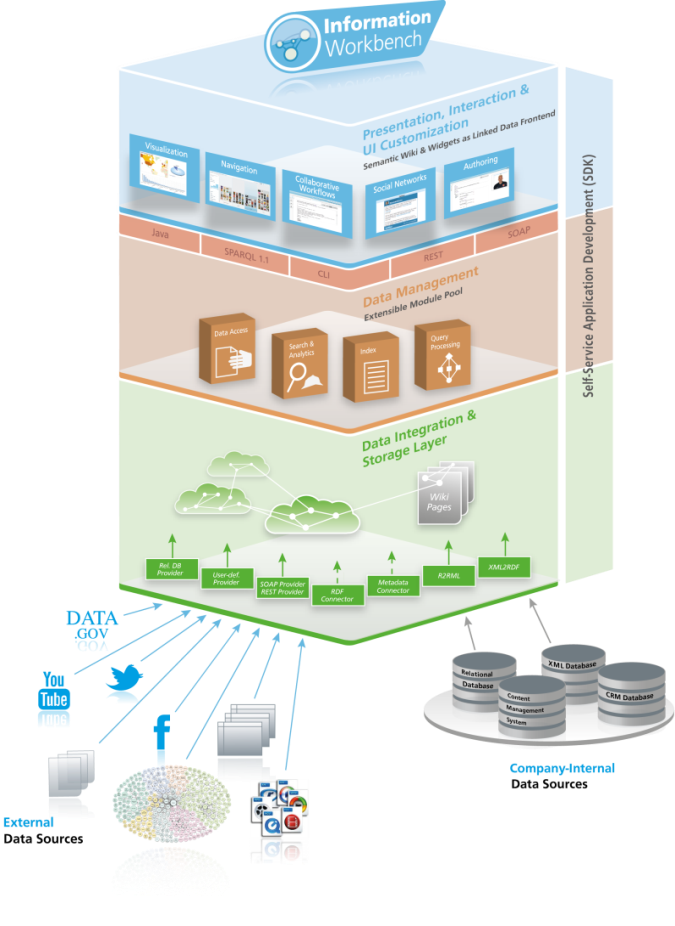
\includegraphics[width=0.9\textwidth]{img/information_workbench_architecture.png}
	\caption{Architecture of the Information Workbench}
	\label{iw_architecture}
\end{figure}

The Information Workbench~\footnote{\url{https://www.fluidops.com/en/products/information_workbench/}} is a high customisable tool to support the building of Linked Data applications, from basic data integration up to rich UI and visualisations. The tool is developed by fluidOps and is published as Community Edition free available and under an Open Source License with a limited selection of capablities and only for non-productive use (educational use, testing, development). The enterprise edition is also available but not for free.

The workbench consists of four layers (see figure~\ref{iw_architecture} for an overview):~\cite{haase2011information}~\cite{gossenainformation}

\begin{itemize}
\item \textbf{Persistence}
Using so-called \emph{providers}, the layers offer capabilities to integrate and convert data from different data source and stores them in a central triple store. Alternatively it also supports virtualised integration of local and public Linked Data sources using a \emph{federation layer}.
\item \textbf{Platform}
On top of the persistence layer the core Platform layer a selection of modules and functionalities covering generic needs of Linked Data applications, the most important are a \emph{Semantic Wiki \& Widget Engin}e, an \emph{User Management \& Access Control}, a \emph{Search \& Analytics Engine} and a \emph{Workflow Engine}.
\item \textbf{SDK} To support customised applications the workbench provides a SDK (Solution Development Kit) for developers to build domain specific applications, including \emph{extensible data providers}, \emph{data management facilities}, modified \emph{ontologies}, \emph{templates}, \emph{widgets} and different APIs for extensive \emph{system configuration}, \emph{rules} and \emph{workflows}.
\item \textbf{Solution}
On top of all layer stands the final solution, the application itself, which is either directly deployed through a RESTful API or over a zipped file for other installation approaches.
\end{itemize}

The resulting application is again customisable by widget and different views, enabling data exploration and visualisation.

\subsection{LDIF – Linked Data Integration Framework}\index{Framework!LDIF}\newacronym{ldif}{LDIF}{Linked Data Integration Framework}

\begin{figure}[htbp]
	\centering
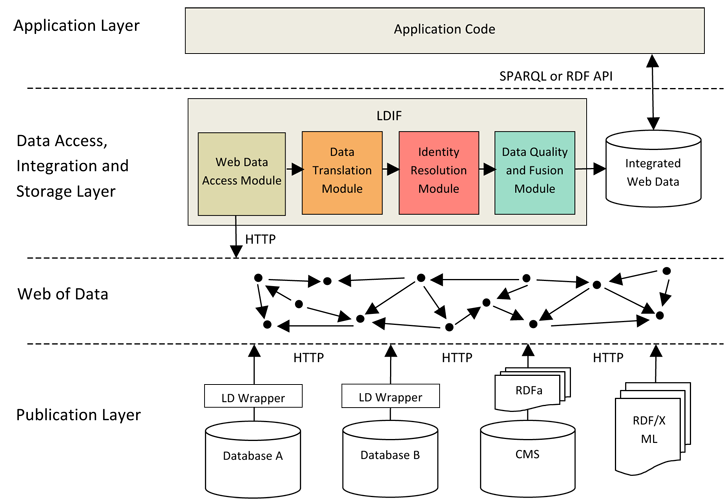
\includegraphics[width=\textwidth]{img/ldif_context.png}
	\caption{LDIF in the context of a LD application}
	\label{ldif_context}
\end{figure}

\begin{figure}[htbp]
	\centering
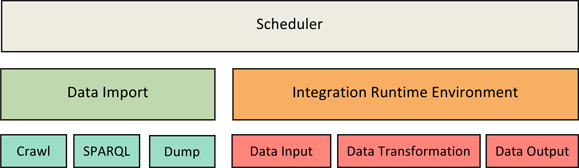
\includegraphics[width=0.8\textwidth]{img/ldif_components.png}
	\caption{Components of LDIF}
	\label{ldif_components}
\end{figure}


LDIF~\footnote{\url{http://ldif.wbsg.de/}} was developed by the University of Mannheim and is published under the terms of the Apache Software License. It is implemented in Scala and aims to translate \emph{"heterogeneous Linked Data from the Web into a clean, local target representation while keeping track of data provenance."}.

From a component perspective, LDIF consists of pluggable modules and a runtime environment, managing the data flows between them. The modules are:~\cite{schultz2011ldif}~\cite{schultz2012ldif}

\begin{itemize}
\item \textbf{Data Access Modules \& Scheduler}
For accessing the data to transform, LDIF provides several ways to import them. These import jobs are managed by a scheduler, which frequently fills a local cache. The module supports Triple/Quade Dump (for RDF/XML, N-Triples, N-Quads and Turtle formats), Crawler (using LDSpider~\footnote{\url{https://github.com/ldspider/ldspider}}) and SPARQL imports.
\item \textbf{Data Translation}
For translating Web data using different vocabularies into a single target vocabulary, LDIF uses the R2R Mapping Language~\footnote{\url{http://wifo5-03.informatik.uni-mannheim.de/bizer/r2r/spec/}}.
\item \textbf{Identity Resolution}
To find different URIs in different data pointing to the same entity, LDIF employs the Silk Link Discovery Framework with the Silk - Link Specification Language (Silk-LSL).
\item \textbf{Data Quality Assessment and Fusion}
For quality assessment, LDIF uses Sieve Data Quality Assessment and Data Fusion Framework~\footnote{\url{http://wifo5-03.informatik.uni-mannheim.de/bizer/sieve/}}.
\item \textbf{Data Output}
In the final step, LDIF write the cleaned data together with the provenance information in a single N-Quads file or without the meta-information in a N-Triples file.
\item \textbf{Runtime Environment} 
As mentioned, the runtime environment manage the data flow between each module, providing an in-memory (fast, but limited scalable), a RDF store (using Apache Jena TDB and SPARQL queries, better scalable for the price of performance) and a Hadoop version.
\end{itemize}

\subsubsection{Silk}\index{Framework!Silk}\label{silk}
Silk~\footnote{\url{http://silkframework.org/}} is \emph{"an open source framework for integrating heterogeneous data sources."} using the declarative Silk - Link Specification Language (Silk-LSL). It generates RDF links between data sets by custom link specifications. There are three different variations:~\cite{isele2010silk}

\begin{itemize}
\item \textbf{Silk Single Machine} generates RDF links between two data items on a single machine.
\item \textbf{Silk MapReduce} is for big scale datasets, using Hadoop and distributes to multiple machines.
\item \textbf{Silk Server} is intended be used as an identity resolution component of as Linked Data consuming application. It provides a REST interface and runs as an HTTP server.
\end{itemize}

For details about the Link Discovery Framework see~\cite{volz2009silk} and~\cite{jentzsch2010silk}, for the server version consult~\cite{isele2010silk}.

\subsection{Eclipse RDF4J (formerly Sesame)}
Eclipse RDF4J~\footnote{\url{http://rdf4j.org/}} (formerly known as Sesame) is \emph{a powerful Java framework for processing and handling RDF data. This includes creating, parsing, scalable storage, reasoning and querying with RDF and Linked Data. It offers an easy-to-use API that can be connected to all leading RDF database solutions.} It can be used as an embedded part of an application or as a stand-alone server.

Originally developed as Sesame by Aduna as part of the "On-To-Knowledge" project (1999-2002), it was official forked into RDF4J. It is licensed under a BSD-style license.

The frameworks comes with many components, like Alibaba, an API for mapping Java classes onto ontologies. The RDF database API is unlikely similar solutions, it consists of stackable interfaces for adding functionality. Next to the intern abstract storage engine (SAIL, Storage and Inference Layer), many other triplestores are supported, like  Ontotext GraphDB, Mulgara, and AllegroGraph

\subsection{Apache Jena}

Apache Jena~\footnote{\url{https://jena.apache.org/}} is \emph{a free and open source Java framework for building Semantic Web and Linked Data applications}. It was originally developed by HP Laboratories and now maintained by the Apache Software Foundation and is licensed under the Apache License 2.0.

The framework provides an API to extract data from and write to RDF, supporting relational databases, RDF/XML, Turtle and Notation 3. In contrast to RDF4J it also supports OWL.

More concrete, Jena can be used to manipulate RDF data, storing them in a triple store and publish it as a SPARQL access point. This HTTP interface is called \emph{Fuseki}, which is in fact a sub-project of Jena and can be also run as stand-alone server using the Jetty web server.

\newpage
\section{Excluded Tools and Projects}\label{excluded}

\subsection{LD-Patterns}\index{Framework!LD-Patterns}
The Linked Data Patterns book by Dodds and Davis (see~\cite{dodds2011linked}) tried to give an overview of existing design pattern regarding LD. But they don't give concrete architectures or architecture relating informations, so this paper will not use its content. But it is suggested, that this design pattern catalogue is used additionally when creating an application.

\subsection{LOD2 Stack}\index{Tools!LOD2 Stack}

The LOD2 stack, introduced by Auer et. al., is \emph{is an integrated distribution of aligned tools which support the whole life cycle of Linked Data from extraction, authoring/creation via enrichment, interlinking, fusing to maintenance.}~\cite{auer2012managing} For this paper the proposed stack of technology was too generic to compare it with other frameworks and the website of the project~\footnote{\url{http://stack.linkeddata.org/lod2//}} was at point of writing this paper offline, therefore it was excluded of this paper.

\subsection{LODUM}\index{Other LOD Projects!LODUM}

Another interesting project is the LODUM project (Linked Open Data University of Münster), the Open Data initiative of the university, hosted at the Institute for Geoinformatics' Semantic Interoperability Lab (MUSIL). The project team has co-initiated both LinkedUniversities.org and LinkedScience.org.

It was excluded for this paper because the project don't provide public documentation of their architecture or any other part of their technical details
\url{http://lodum.de/}

\subsection{Synth and SHDM}\index{Framework!Synth}

\begin{figure}[htbp]
	\centering
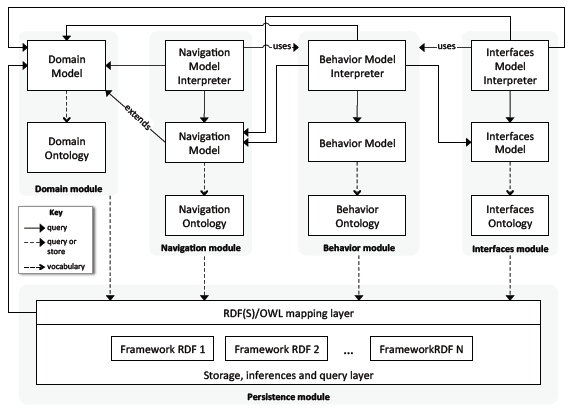
\includegraphics[width=\textwidth]{img/synth-concept.png}
	\caption{Concept of the Synth Architecture}
	\label{synth_concept}
\end{figure}

Synth~\footnote{\url{http://www.tecweb.inf.puc-rio.br/synth}} is a development environment for building SHDM~\footnote{\url{https://www.w3.org/2005/Incubator/model-based-ui/wiki/SHDM_-_Semantic_Hypermedia_Design_Method}} (Semantic Hypermedia Design Method) modelled applications, providing a set of modules, receiving SHDM generated models. Synth comes with a web browser GUI for adding and editing these models. A conceptual view of the architecture can be seen in figure~\ref{synth_concept}, where the dashed boxes are modules and the whites boxes insides the module components.~\cite{desynth} The authors de Souza Bomfim and Schwabe describe in two papers, how a Linked Data application can be build with the environment: ~\cite{desynth} and~\cite{de2011design}.

Since their description is very abstract and there are no further documentations of the tool, it was excluded for this paper. 
\chapter{Criteria (RQ2)}\label{criteria}

Since there are a wide variety of solutions, it is hard to find a set of criteria which can be applied to all in the same way in order to compare them. Therefore this paper will use 4 different criteria groups to ensure higher cover of them, even in case some of the criteria might not be applicable. Otherwise a comparison will be not possible.

\section{Criteria Group 1: Criteria from previous study}

\begin{table}[htb]
\centering
\begin{tabular}{|l|l|l|}
\rowcolor[HTML]{EFEFEF} 
\hline
\textbf{Criteria} & \textbf{Scala} & \textbf{Explanation}                                 \\ \hline
Maintainability   & +/-            & How much effort needs the maintenance?                        \\ \hline
Data Freshness    & yes/ no        & Can it deal with new data?                        \\ \hline
Flexibility       & yes/ no        & \begin{tabular}[c]{@{}l@{}}Can it deal with heterogenous and/or legacy data? \\ Can it deal with changes in the ontology?\end{tabular} \\ \hline
\end{tabular}
\caption{Criteria group 1}
\label{tbl_cr_1_scala}
\end{table}

From a previous study~\cite{baronyai_publishing_2016} conducted by the author, users at TU Wien are expecting and requesting from a LOD application: \textbf{clear data ownership}, management of \textbf{data freshness} and \textbf{data quality} and \textbf{maintenance}. Since data ownership is a concern of organisation and cannot be clarified by a tool, data freshness, data quality and maintainability are introduced as criteria. Since data quality is a very generic term, it will be used as criteria category. Additionally a concern of the stakeholders from the paper was how to deal with legacy data, therefore flexibility is included to Data quality.

The resulting criteria can be seen in table~\ref{tbl_cr_1_scala}.

\section{Criteria Group 2: Usability}

\begin{table}[htb]
\centering
\begin{tabular}{|l|l|l|}
\hline
\rowcolor[HTML]{EFEFEF} 
\textbf{Criteria} & \textbf{Scala} & \textbf{Explanation}                                                                                                \\ \hline
Effectiveness     & +/-            & \begin{tabular}[c]{@{}l@{}}How well do the users achieve their goals using the system? \\ (good/bad)\end{tabular}   \\ \hline
Efficiency        & +/-            & \begin{tabular}[c]{@{}l@{}}What resources are consumed in order to achieve their goals? \\ (less/much)\end{tabular} \\ \hline
Satisfaction      & +/-            & \begin{tabular}[c]{@{}l@{}}How do the users feel about their use of the system? \\ (good/bad)\end{tabular}          \\ \hline
Security          & +/-            & \begin{tabular}[c]{@{}l@{}}How well is security ensured? \\ (good/bad)\end{tabular}                                 \\ \hline
Learnability      & +/-            & \begin{tabular}[c]{@{}l@{}}How much time is needed to learn the system? \\ (less/much)\end{tabular}                 \\ \hline
\end{tabular}
\caption{Criteria Group 2: Usability}
\label{tbl_cr_2_scala}
\end{table}

In every software application and especially solutions designed for end-users, usability is a huge and very important point these days. There are many definitions and measurements, ISO and other proposed models, trying to classify and define usability. This paper will use an enhanced ISO model, proposed by Abran et.al.~\cite{abran2003usability}. Since the goal of this paper is not a complete usability analysis of the tools/frameworks and the variety of the chosen tools is too wide, the analysis of these aspect will be more of a general type. Abran et.al. are proposing various measurements for the different categories of their model, the interested reader might use them for a detailed analysis. For this paper, these measurements will only be used as a guideline to estimate an assessment for the tools.

The model can be seen in table~\ref{tbl_cr_2_scala}

\section{Criteria Group 3: Data formats}

An important aspect for the final decision for one of the tools can be the supported data format. It might be an (external) requirement or resulting from the fact of existing data. Since this highly depends on the context and the use case, this criteria will not be rated in any way, this paper will only line out the supported data formats.

\section{Criteria Group 4: Linked Data Publishing Checklist}

\begin{table}[htb]
\centering
\begin{tabular}{|l|}
\rowcolor[HTML]{EFEFEF} 
\hline
\multicolumn{1}{|c|}{\textbf{Criteria}}                        \\ \hline
Does your data set links to other data sets?                   \\ \hline
Do you provide provenance metadata?                            \\ \hline
Do you provide licensing metadata?                             \\ \hline
Do you use terms from widely deployed vocabularies?            \\ \hline
Are the URIs of proprietary vocabulary terms dereferenceable?  \\ \hline
Do you map proprietary vocabulary terms to other vocabularies? \\ \hline
Do you provide data set-level metadata?                        \\ \hline
Do you refer to additional access methods?                     \\ \hline
\end{tabular}
\caption{Criteria Group 4: Linked Data Publishing Checklist}
\label{tbl_cr_4_scala}
\end{table}

Since the whole paper is about Linked Data, it is important to analyse not only the tools itself but also the resulting LDs. In order to do that, the Linked Data Publishing Checklist by Heath et.al.~\cite{heath2011linked} will be used. Another alternative could be the the LOD defintion itself by Tim Berners-Lee~\cite{berners2006linked}, but this paper will presume, that a L(O)D tool will produce valid L(O)D. As one can expect from a checklist, the rating for this criteria will be only fulfilled/not fulfilled.

The checklist can be seen in table~\ref{tbl_cr_4_scala}

\section{End result}

Since this paper is designed to be used as a help for decisions, the aim can not be to find the "best" solution, therefore there will not be such a thing like an end result. E.g. for some situation a solution with bad usability can be more appropriate because of the supported data formats than a solution with a higher overall rating.

\begin{table}[htb]
\begin{tabular}{|l|l|}
\rowcolor[HTML]{EFEFEF} 
\hline
\textbf{Criteria group}             & \multicolumn{1}{c|}{\textbf{Criteria}} \\ \hline
\multirow{3}{*}{Group 1}            & Maintainability                        \\ \cline{2-2} 
                                    & Data Freshness                         \\ \cline{2-2} 
                                    & Flexibility                            \\ \hline
\multirow{5}{*}{Group 2: Usability} & Effectiveness                          \\ \cline{2-2} 
                                    & Efficiency                             \\ \cline{2-2} 
                                    & Satisfaction                           \\ \cline{2-2} 
                                    & Security                               \\ \cline{2-2} 
                                    & Learnability                           \\ \hline
Group 3: Data formats               & Data formats                           \\ \hline
\begin{tabular}[c]{@{}l@{}}Group 4: LD Publishing \\ Checklist\end{tabular}    & LD Publishing Checklist                \\ \hline
\end{tabular}
\centering
\caption{Complete Criteria Catalogue}
\label{tbl_cr_all}
\end{table}
\chapter{Comparison (RQ3)}\label{comparison}

It this section the comparison itself will be done. In order to do that, first in section~\ref{comp_classification} the classification introduced in section~\ref{classification} will be applied the found solution. Then in section~\ref{comparison} the criteria defined in section~\ref{criteria} will be applied for each of them, divided in the defined groups. The summary in section~\ref{comp_summary} will then give in overview of the done comparison. 

An overview of the solutions to compare can be seen as recap in table~\ref{tb:cmp_overview}, in order to simplify the following tables, each of the solutions is given an ID to refer.

\begin{table}[htbp]
\centering
\begin{tabular}{|l|l|}
\hline
\rowcolor[HTML]{EFEFEF} 
\textbf{ID} & \textbf{Framework}    \\ \hline
1           & Euclid Project        \\ \hline
2           & LUCERO                \\ \hline
3           & Linked Data book      \\ \hline
4           & D2RQ Platform         \\ \hline
5           & Information Workbench \\ \hline
6           & \begin{tabular}[c]{@{}l@{}}Linked Data \\ Integration Framework\end{tabular}                  \\ \hline
7           & Eclipse RDF4J         \\ \hline
8           & Apache Jena           \\ \hline
\end{tabular}
\caption{Overview of the solutions}
\label{tb:cmp_overview}
\end{table}

\section{Classification}~\label{comp_classification}

\begin{table}[htbp]
\centering
\resizebox{\textwidth}{!}{%
\begin{tabular}{|c|c|c|c|c|c|l|}
\hline
\rowcolor[HTML]{EFEFEF} 
\textbf{ID} & \multicolumn{1}{c|}{\textbf{\begin{tabular}[c]{@{}c@{}}Arch-\\ itecture\end{tabular}}} & \multicolumn{1}{l|}{\textbf{\begin{tabular}[c]{@{}l@{}}Full-\\ Stack\end{tabular}}} & \multicolumn{1}{l|}{\textbf{\begin{tabular}[c]{@{}l@{}}Present-\\ ation \\ layer\end{tabular}}} & \multicolumn{1}{l|}{\textbf{\begin{tabular}[c]{@{}l@{}}Business \\ Layer\end{tabular}}} & \multicolumn{1}{l|}{\textbf{\begin{tabular}[c]{@{}l@{}}Data \\ Access \\ Layer\end{tabular}}} & \textbf{Note} \\ \hline
\textbf{1} & x &  &  & x & x &  \\ \hline
\textbf{2} & x &  &  & x & x &  \\ \hline
\textbf{3} & x &  &  & x & x &  \\ \hline
\textbf{4} &  &  & x & x & x & \begin{tabular}[c]{@{}l@{}}D2R Server includes HTML \\ view and SPARQL endpoints\end{tabular} \\ \hline
\textbf{5} &  & x &  &  &  &  \\ \hline
\textbf{6} &  &  &  & x & x &  \\ \hline
\textbf{7} &  &  &  & x & x &  \\ \hline
\textbf{8} &  &  & x & x & x & \begin{tabular}[c]{@{}l@{}}Provides optionally SPARQL \\ endpoints and stand-alone \\ server with Jetty\end{tabular} \\ \hline
\end{tabular}
}
\caption{Classification}
\label{tbl:cmp_classification}
\end{table}

\section{Criteria Group 1: Criteria from previous study}

\begin{table}[htbp]
\centering
\resizebox{\textwidth}{!}{%
\begin{tabular}{|c|c|c|c|l|}
\hline
\rowcolor[HTML]{EFEFEF} 
\textbf{ID} & \textbf{\begin{tabular}[c]{@{}l@{}}Maintain\\ -ability\end{tabular}} & \textbf{\begin{tabular}[c]{@{}l@{}}Data \\ Freshness\end{tabular}} & \textbf{Flexibility} & \textbf{Note} \\ \hline
\textbf{1}  & +                                                                     & yes*                                                                 & yes*                                                              & *depending on implementation     \\ \hline
\textbf{2}  & ?*                                                                    & yes                                                                  & yes*                                                              & *further investigations required \\ \hline
\textbf{3}  & +                                                                     & yes*                                                                 & yes*                                                              & *depending on implementation     \\ \hline
\textbf{4}  & +                                                                     & yes                                                                  & yes*                                                              & *depending on configuration      \\ \hline
\textbf{5}  & ?*                                                                    & yes*                                                                 & yes*                                                              & *depending on configuration      \\ \hline
\textbf{6}  & +                                                                     & yes                                                                  & yes*                                                              &                                  \\ \hline
\textbf{7}  & $\sim$*                                                               & ?*                                                                   & yes*                                                              & *depending on implementation     \\ \hline
\textbf{8}  & $\sim$*                                                               & ?*                                                                   & yes*                                                              & *depending on implementation     \\ \hline
\end{tabular}
}
\caption{Comparison Criteria Group 1}
\label{tbl_comp_gr_1}
\end{table}

\subsection*{1: Euclid Project} 
Since the Euclid Project is very generic, the Data Freshness and Flexibility totally depends on how the concepts are implemented in an application. If the concepts are correctly implemented, Maintainability is probably well supported, since the three-layered architecture is widely recognised for it. For Data Freshness and Flexibility, the implementation needs to be done focused on it, in order to achieve it, since the project does it not explicitly.

\subsection*{2: LUCERO}
The project supports Data Freshness by its Updaters and Schedulers, and can react to ontology changes by its Entity Name System. But it is unclear, how well it supports Maintainability, further investigations are required, which exceed the scope of this paper.

\subsection*{3: Linked Data book}
Similar to the Euclid Project, the Data Freshness and Flexibility is possible well supported, but depends on the implementation. It is also not an explicit focus. Maintainability again is inherit of the concept.

\subsection*{4: D2RQ Platform}
The D2RQ Mapping Language can flexibly handle heterogeneous data as well as legacy data, the quality of Data Freshness depends on the configuration but is itself inherit of the concept.

\subsection*{5: Information Workbench}
Since the Workbench is designed to easily integrate different datasources, it can handle legacy data and ontology changes relatively good, depending on custom configurations. It might be a challenge to find the correct configurations, but the provided documentation well done.

\subsection*{6: LDIF}
LDIF is explicit designed to handle various data sources and vocabularies, mapping them to an uniform vocabulary. The framework further provides scheduler to keep the data as fresh as needed (running hourly, daily etc.)

\subsection*{7: Eclipse RDF4J}
All three criteria are highly depending on the implementation of the framework and therefore how maintainability, freshness and flexibility are handled. The framework itself does only interact with a repository (read/write), which can potential be filled by another application which handles freshness and flexibility. Maintainability could be a bit tricky in this situation, if the other application is out of control of the RDF4J implementation.

\subsection*{8: Apache Jena}
Jena is very similar to RDF4J, all statements there are valid for Jena too.

\subsection{Summary Group 1}
Most of the solutions are supporting all data freshness and flexibility although most of them depending on the concrete implementation or configuration of the application. Only LDIF have a clear support of especially data freshness and flexibility. Maintainability is a critical point for most of the solutions.

\section{Criteria Group 2: Usability}

\begin{table}[htbp]
\centering
\resizebox{\textwidth}{!}{%
\begin{tabular}{|l|c|c|c|c|c|l|}
\hline
\rowcolor[HTML]{EFEFEF} 
\textbf{ID} & \multicolumn{1}{l|}{\cellcolor[HTML]{EFEFEF}\textbf{Effectiveness}} & \multicolumn{1}{l|}{\cellcolor[HTML]{EFEFEF}\textbf{Efficiency}} & \multicolumn{1}{l|}{\cellcolor[HTML]{EFEFEF}\textbf{Satisfaction}} & \multicolumn{1}{l|}{\cellcolor[HTML]{EFEFEF}\textbf{Security}} & \multicolumn{1}{l|}{\cellcolor[HTML]{EFEFEF}\textbf{Learnability}} & \textbf{Note}                                                                     \\ \hline
\textbf{1}  & N.A.                                                                & N.A.                                                             & N.A.                                                               & -                                                              & +                                                                  & \begin{tabular}[c]{@{}l@{}}Not applicable, \\ good documentation\end{tabular}     \\ \hline
\textbf{2}  & N.A.                                                                & N.A.                                                             & N.A.                                                               & -                                                              & -                                                                  & \begin{tabular}[c]{@{}l@{}}No UI, no Security, \\ bad documentation\end{tabular}  \\ \hline
\textbf{3}  & N.A.                                                                & N.A.                                                             & N.A.                                                               & -                                                              & +                                                                  & \begin{tabular}[c]{@{}l@{}}Not applicable, \\ good documentation\end{tabular}     \\ \hline
\textbf{4}  & +                                                                   & +                                                                & +                                                                  & -                                                              & +                                                                  & \begin{tabular}[c]{@{}l@{}}Good documentation \\ and UI, no security\end{tabular} \\ \hline
\textbf{5}  & +                                                                   & +                                                                & +*                                                                 & +                                                              & +*                                                                 & \begin{tabular}[c]{@{}l@{}}* "easy to learn, \\ hard to master"\end{tabular}      \\ \hline
\textbf{6}  & N.A.                                                                & N.A.                                                             & N.A.                                                               & -                                                              & +                                                                  & \begin{tabular}[c]{@{}l@{}}Not applicable, \\ good documentation\end{tabular}     \\ \hline
\textbf{7}  & N.A.                                                                & N.A.                                                             & N.A.                                                               & $\sim$                                                         & +                                                                  & \begin{tabular}[c]{@{}l@{}}Not applicable, \\ good documentation\end{tabular}     \\ \hline
\textbf{8}  & N.A.                                                                & N.A.                                                             & N.A.                                                               & +                                                              & +                                                                  & \begin{tabular}[c]{@{}l@{}}Not applicable, \\ good documentation\end{tabular}     \\ \hline
\end{tabular}%
}
\caption{Comparison Criteria Group 2: Usability}
\label{tbl_comp_gr_2}
\end{table}

\subsection*{1: Euclid Project}
Since the Usability totally depends on the implemented application, no general statements can be given here. Security is not explicit. The documentation is very good.

\subsection*{2: LUCERO}
The project does not support an explicit UI, therefore Usability is hard to evaluate. It also does not have any integrated security. The documentation is old and possible outdated, therefore learnability of the system is relatively bad.

\subsection*{3: Linked Data book}
Again, similar to Euclid, the Usability strongly depends on the implementation and is therefore not applicable. Security is not explicit.

\subsection*{4: D2RQ Platform}
The D2RQ server provides a basic but good readable UI. The documentation of the whole platform is very good. Security is not part of the project.

\subsection*{5: Information Workbench}
The workbench has a very well designed UI, supporting the user to achieve their tasks relatively simple. The system is very good readable, enabling the user to explore the functionality and fulfilling their task. The according documentation is well done for "standard" users, but might be not enough for advanced development. Security is per default activated.

\subsection*{6: LDIF}
LDIF does not have an explicit UI, therefore there can be no assessment of it done. Security is not part of the LDIF concept. The documentation is well done, but covers only simple topics, which could be problematic when running into problems while using the framework.

\subsection*{7: Eclipse RDF4J}
The framework provides a simple UI for the RDF4J server and workbench for managing the repositories, but using RDF4 means writing Java Code. Therefore UI can not be topic of examination here. The RDF4J repositories have simple user management, but are handled per default by plain text cookies in the browser. The documentation is detailed and in good condition.

\subsection*{8: Apache Jena}
Again, all statements from RDF4J are valid for Jena too. But in contrast to RDF4J Jena uses Apache Shiro for security. The server for Jena is called Fuseki.

\subsection{Summary Group 2}
Most of the solutions does not support an UI, except D2RQ and the information workbench. Security is only explicit mentioned in the information workbench and Apache Jena, RDF4J's default security is very basic. All solutions except LUCERO provide a good documentation.

\section{Criteria Group 3: Data formats}

\begin{table}[htbp]
\centering
\resizebox{\textwidth}{!}{%
\begin{tabular}{|c|l|l|}
\hline
\rowcolor[HTML]{EFEFEF} 
\textbf{Solution} & \textbf{Data formats}                                                                                                                        & \textbf{Note}                                                                                                                                                                  \\ \hline
\textbf{1}        & Potential every possible format                                                                                                              & \begin{tabular}[c]{@{}l@{}}Every format needs its own \\ wrapper/consumer\end{tabular}                                                                                         \\ \hline
\textbf{2}        & Default RSS \& XML                                                                                                                           & \begin{tabular}[c]{@{}l@{}}Additional data formats need \\ custom extractors\end{tabular}                                                                                      \\ \hline
\textbf{3}        & \begin{tabular}[c]{@{}l@{}}Recipes for RDF, XML, HTML, \\ relational databases, Wrapper\end{tabular}                                         &                                                                                                                                                                                \\ \hline
\textbf{4}        & Only relational databases                                                                                                                    &                                                                                                                                                                                \\ \hline
\textbf{5}        & \begin{tabular}[c]{@{}l@{}}Table-base (csv, excel, groovy, \\ jdbc, rest, tsv, sparql etc), \\ tree-based (xml, json, etc), RDF\end{tabular} & \begin{tabular}[c]{@{}l@{}}Each data source needs a \\ configured data provider \\ which provides R2RML \\ (tabular datasources) and \\ XML mappings to RDF (see)\end{tabular} \\ \hline
\textbf{6}        & \begin{tabular}[c]{@{}l@{}}N-Quads dumps, RDF/XML, \\ N-Triples, Turtle dumps,\\ dereferenced URIs, SPARQL\end{tabular}                      & \begin{tabular}[c]{@{}l@{}}Using LDSpider for \\ URI crawl import\end{tabular}                                                                                                 \\ \hline
\textbf{7}        & Only RDF                                                                                                                                     &                                                                                                                                                                                \\ \hline
\textbf{8}        & Only RDF \& OWL                                                                                                                              &                                                                                                                                                                                \\ \hline
\end{tabular}
}
\caption{Comparison Criteria Group 3: Data formats}
\label{tbl_comp_gr_3}
\end{table}

\subsection*{1: Euclid Project}
The Euclid Project does theoretically supports every kind of formats, since it requires the developer to write a consumer for each data source, additionally enhanced by a wrapper to transform the data to RDF.

\subsection*{2: LUCERO}
Per default, the project supports only RSS and XML, but it provides also mechanism to integrate additional data extractors to the system, to enable addition data formats.

\subsection*{3: Linked Data book}
The book provides recipes for RDF, XML, HTML, relational databases and wrapper for existing applications and Web APIs. Additional data formats can probably integrated by adopting the recipes.

\subsection*{4: D2RQ Platform}
The scope of the platform are only the integration of relational databases.

\subsection*{5: Information Workbench}
The workbench does support a wide range of data format. For each data source, a data provider has to be configured. For table- and tree-based data formats are mappings available to transform the data to RDF.

\subsection*{6: LDIF}
LDIF provides four types of import jobs: Quad (import N-Quads dumps), Triple (import RDF/XML, N-Triples or Turtle dumps), Crawl (import by dereferencing URIs as RDF data, using the LDSpider Web Crawling Framework) and SPARQL Import Job (import by querying a SPARQL endpoint)

\subsection*{7: Eclipse RDF4J}
The framework is mainly meant for working with data from a RDF repository and not explicit for putting/creating data in it in the first place. 

\subsection*{8: Apache Jena}
Jena is also developed with the focus of accessing data rather than creating the data store, therefore only RDF and additionally OWL are supported.

\subsection{Summary Group 3}
The solutions offer a wide range of data types in total, the Euclid Project and the LD book provide recipes for various data types, the Information Workbench does this out-of-the-box. D2RQ, RDF4J and Jena are specialised solutions, focusing only on single data types.

\section{Criteria Group 4: Linked Data Publishing Checklist}

\begin{table}[htbp]
\centering
\resizebox{\textwidth}{!}{%
\begin{tabular}{|l|c|c|c|c|c|c|c|c|}
\hline
\rowcolor[HTML]{EFEFEF} 
\textbf{ID}                                              & \textbf{1} & \textbf{2} & \textbf{3} & \textbf{4} & \textbf{5} & \textbf{6} & \textbf{7} & \textbf{8} \\ \hline
Does your data set links to other data sets?                   & x          & x          & x          & x          & x          & x          & ?          & ?          \\ \hline
Do you provide provenance metadata?                            & x          & ?          & x          & x          & x          & x          & x          & x          \\ \hline
Do you provide licensing metadata?                             & x          & ?          & x          & x          & x          & x          & x          & x          \\ \hline
Do you use terms from widely deployed vocabularies?            & x          & x          & x          & x          & x          & x          & ?          & ?          \\ \hline
Are the URIs of proprietary vocabulary terms dereferenceable?  & x          & x          & x          & x          & x          & x          & ?          & ?          \\ \hline
Do you map proprietary vocabulary terms to other vocabularies? & x          & x          & x          & x          & x          & x          & -          & -          \\ \hline
Do you provide data set-level metadata?                        & x          & ?          & x          & x          & x          & x          & x          & x          \\ \hline
Do you refer to additional access methods?                     & x          & -          & x          & x          & x          & x          & ?          & ?          \\ \hline
\end{tabular}
}
\caption{Comparison Criteria Group 4: Linked Data Publishing Checklist}
\label{tbl_comp_gr_4}
\end{table}

\subsection*{1: Euclid Project}
Since of its generic nature, possible every point of the checklist can be fulfilled depending on the implementation. But the architecture does not require any of the points.

\subsection*{2: LUCERO}
LUCERO supports interlinking of data and through its Entity Name System different vocabularies. Since its bad documentation, it is unclear, if any metadata are provided (assumably not).

\subsection*{3: Linked Data book}
Since Heath et al. propose the checklist in this book, it is also implicit and explicit integrated into the described solutions.

\subsection*{4: D2RQ Platform}
The D2RQ server provides comprehensive support for metadata, easy customizable by templates. The D2RQ Mapping language is very powerful in handling and mapping various kinds of vocabulary.

\subsection*{5: Information Workbench}
The workbench does support metadata, licensing metadata can be provided by custom implementations. Interlinking is as well supported as different kinds of vocabularies.

\subsection*{6: LDIF}
The framework implicit provides provenance next to the triple store, links to other data sets and maps proprietary vocabulary terms. The LD book explicit mentions LDIF as good example, therefore it can easily be assumed, that the checklist is fulfilled.

\subsection*{7: Eclipse RDF4J}
Again, same as the Euclid Project, nearly every point of the checklist could be fulfilled by an implementation, especially the points about meta data. The schema/vocabulary/structure can be independent of the application and managed by another one, therefore it is out of the scope of RDF4J.

\subsection*{8: Apache Jena}
For Jena are the same arguments than for RDF4J valid: meta data are depended on the implementation, schema/vocabulary/structure can be out of the scope.

\subsection{Summary Group 4}
The checklist is overall well supported although it, again, is depending on the implementation of some of the solutions like Euclid, RDF4J or Jena. The last two are not managing the schema/vocabulary/structure by themselve, therefore the checklist is only partially applicable.

\section{Summary}\label{comp_summary}

Overall the concept of having multiple criteria worked, since some solution could not be evaluated in some categories like Usability. But in the overall view, the criteria helped to find a standardised way to describe the solutions and compare them. In the following section, the evaluation of each solution will be summarized to have a better overview.

\subsection*{1: Euclid Project}
Since the Euclid Project does only provide a generic architecture, most of the criteria are not directly applicable and are depending on the concrete implementation. Correctly applied it does however supports directly or indirectly maintainability, data freshness, flexibility, various kinds of data formats and the complete LD checklist. The architecture has no focus, neither explicit nor implicit, on security, therefore it needs to be done additionally if required. The documentation of the architecture is outstanding and very good done.
Comparing to the other solutions, Euclid provides structures how other solutions or custom implementation can interact with each other. It can also be used as blueprint when combining other solutions.

\subsection*{2: LUCERO}
LUCERO is on one hand overall bad documented and outdated. On the other hand, it does support data freshness and flexibility per default due its mechanisms and can support various data formats by custom extractors. But due the first facts, it is not recommended any more to use LUCERO in a real application.

\subsection*{3: Linked Data book}
The summary for the LD book architecture is similar structured to the one of the Euclid project: good documentation but overall very generic. It can support maintainability, data freshness and flexibility if well implemented. The documentation is good and does include various recipes of data formats.
A possible use case for it is the same as for Euclid: as blue print for combining other solutions.

\subsection*{4: D2RQ Platform}
The D2RQ is as mentioned a specialised tool for relational databases. According to it, it has only limited data format supports. But due its simple structure and focused usage, data freshness, maintainability and flexibility can be assured. D2RQ includes a good UI and documentation.
This solution is ideal for a very specific use case, requiring only a relational database to publish as L(O)D, but solving it as an all-in-one solution without the need of further tool integration.

\subsection*{5: Information Workbench}
The Information Workbench is an all-in-solution, rich with functions and with a wide range of supported data formats. It can be used as a full stack solution with UI, integrating different data repositories. The documentation is well done but simple written, resulting maybe into problems handling more complex problems.
The Workbench is ideal for an use case involving multiple data sources. For smaller use cases, it could be an overloaded solution.

\subsection*{6: LDIF}
LDIF is due its concept on the one side a very flexible framework for handling different data sources with a wide range of vocabulary which also provides mechanism for keeping the retrieved data fresh. On the other hand the specialisation leads to a specific focus resulting in a limit number of supported data formats.
An use case for LDIF can be managing different data sources on base of RDF, SPARQL or something similar. Since it is not an all-in-one solution, it can/should be used in combination with another tool responsible for exposing the data to the web.

\subsection*{7: Eclipse RDF4J}
RDF4J is completely different to the other investigated solutions, since it is a Java framework, requiring the developer to implement the given APIs. It is designed to handle a given repository and work with its data and/or expose them to the web. If an use case requires to publish data \emph{not} in RDF format, it could be good idea to use RDF4J in combination with a tool like LDIF.

\subsection*{8: Apache Jena}
As already mentioned Jena is similar to Sesame, but with the addition, that it provides support for OWL. It is also designed to handle a given repository and might be used in combination with something like LDIF.
\chapter{A Case Study Of Applying The Evaluation Framework At TU Wien (RQ4)}\label{ch:tuwien}

In this section, the paper tries to answer research question 4: What a LD solution for TU Wien might look like.

\section{General Considerations}
In order to answer the question, it is important to give a context, since it is difficult respectively impossible to give a general, generic solution. In the following sections, three possible scenarios will be proposed, which can be a possible use case at TU Wien. For each scenario the requirement will be defined and a solution assigned.

From the previous study~\cite{baronyai_publishing_2016} conducted by the author the following requirements are important for the TU stakeholders:

\begin{itemize}

\item \textbf{Maintainable}: \\
A LD application at TU Wien has to be easily maintainable. Citing stakeholders from the previous study, it "simply has to work without having to care about continuously".

\item \textbf{Fresh Data}: \\
It was important for the stakeholders, that the provided data are up-to-date.

\item \textbf{Legacy Data}: \\
A possible solutions for TU Wien has necessarily handle legacy data since this are the kind of data, that are candidates for publishing.

\end{itemize}

These requirements are therefore valid for each following scenario, meaning that criteria group 1 is higher weighted than the other groups. A solution, that does not full-fill one of this criteria, will not be take account of at all.

\section{Situations \& Requirements}

As mentioned, to answer the research question, the context needs to be specified. This will be done by analysing the stakeholders (already done by the previous study). These findings will then be combined to scenarios.

\subsection{Stakeholders}

\textbf{Researcher} are interested in an easy access to the publications of the university and publications in general as well as an easy access to resources for their research subject. They need to \emph{use} the data without further work in order to focus on their actual daily work. That also applies if the research is teaching at the university: in order to use an application, either by accessing it or providing data to it, it would be rejected by the stakeholders, if it means significant more work. But since they are used to technical work, the inhibition threshold to use a LD application is lower than for the administration staff.

\textbf{Administration staff} is more a subject of data source than of data user since they are holding a lot of interesting data. But on the other hand, the 
inhibition threshold is higher than for the researcher since the technical experience is at average lower. Therefore the argument of an "easy-to-use" of the previous stakeholder group is even more valid here.

\textbf{Students} are mainly data consumer and therefore more concerned with the frontend of a possible application. This group can build application that are consuming the published data.

\subsection{Situations}

In the following sections will describe possible scenarios at TU Wien, how and which data are going to be published. There are two base scenarios: publishing a single data source and building a platform with various data sources. The second one will be additional split.

\subsubsection{Situation 1: Specialised Single Solution}

Only one or a small number of data source(s) needs to be published. The application has to be specific done for this data set. The project is small scaled and can be done quickly. A possible data source could be the publication database. This scenario can be used as a demonstration, how to \emph{consume} Linked Open Data, but it is not advisable to use this approach if any other data source might be published in the future, since this scenario is \emph{not} scalable

\textbf{Requirement}
\begin{itemize}
\itemsep0pt
\item small scale
\item small number of data sets
\item specialised solution
\item simple
\end{itemize}

\subsubsection{Scenario 2: Function-rich Platform}

A comprehensive platform is needed, which covers a variety of data of different formats, including relational data as well as semi-structured data like XML. The project is medium scaled, the platform shall be able to handle data TU wide and is not only for internal purpose but also for external usage. Additional, the platform has to offer meta data, documentation and performance data. The solution has to be easy to use and implement. Licensing or Open Source does not play a role. 

\textbf{Requirement}
\begin{itemize}
\itemsep0pt
\item various kinds of data sets (in number and formats)
\item medium scale
\item platform with additional features
\item easy to use/implement
\end{itemize}

\subsubsection{Scenario 3: Complete Controlled Platform}

Similar to scenario 2, it is necessary to build platform combining different kinds of data sources. But in contrast, full control over the platform and the technology stack is necessary and no licensing is wanted, an Open Source Solution is necessary. In exchange, the requirement "easy to use/implement" is relaxed, but still relevant.

\textbf{Requirement}
\begin{itemize}
\itemsep0pt
\item various kinds of data sets (in number and formats)
\item medium scale
\item platform with additional features
\item no licensing
\item Open Source
\end{itemize}

\section{Proposed Solutions}

\subsection{Scenario 1: Specialised Single Solution}

There are two solution thinkable:

\paragraph{Option 1: D2RQ} can be a solution for this situation. It provides a simple mapping of a given data set and a method of publishing with the D2R Server. The project can be fast implemented and be ready. Other data sets may be added. Since D2RQ only handles relational data, this approach is not suitable for semi-structured data.

\paragraph{Option 2: A combination of Jena/RDF4J with Euclid and LDIF} can be used to publish he given data. The Euclid architecture (assuring maintainability) can be used as a blueprint to implement an application using either the Apache Jena or Eclipse RDF4J framework. If a mapping is needed, LDIF can be used additionally. This solution is far more extensive than using D2RQ, but on the other hand more flexible and customisable. The scope can be controlled by defining the limits, specially by economizing the UI, but be aware that this approach can result in an lesser usability and the scope might be too big for this situation.

\subsection{Scenario 2: Function-rich Platform}

For this scenario is the \textbf{Information Workbench} suitable. The tool can integrate different kinds of data sources, combine the access points to a platform and providing additional features over modules. The implementation can be done relatively simple and fast. However, it needs a licensing if used outside an educational scope.

\subsection{Scenario 3: Complete Controlled Platform}

For this scenario no all-in-one solution of the proposed tools is suitable, instead the platform has to be developed by using a framework like \textbf{Jena or RDF4J} in combination with the \textbf{Euclid Project architecture}, similar to the solution proposed situation 1. If a mapping to an unified vocabulary is needed, \textbf{LDIF} can also be used. This project will probably consume more time and will have a bigger scope than the solution of situation 2. But on the other hand, this approach offers more customisation options.

\section{Summary}

\begin{table}[hbtp]
\centering
\resizebox{\textwidth}{!}{%
	\begin{tabular}{|l|l|l|}
		\hline
		\rowcolor[HTML]{EFEFEF} 
		\textbf{Scenario} & \textbf{Requirement} & \textbf{Solution} \\ \hline
		%%
		\textbf{\begin{tabular}[c]{@{}l@{}}Specialised \\ Single Solution\end{tabular}} & 
		\begin{tabular}[c]{@{}l@{}}
			-) small scale \\ 
			-) small number of data sets \\ 
			-) specialised solution \\ 
			-) simple
		\end{tabular} & 
		\begin{tabular}[c]{@{}l@{}}
			-) Option 1: D2RQ \\ 
			-) Option 2: Jena + Euclid \\ (+ LDIF)
		\end{tabular} \\ \hline
		%%
		\textbf{\begin{tabular}[c]{@{}l@{}}Function-rich \\ Platform\end{tabular}} & 
		\begin{tabular}[c]{@{}l@{}}
			-) various kinds of data sets \\ (in number and formats) \\ 
			-) medium scale \\ 
			-) platform with additional features \\ 
			-) easy to use/implement
		\end{tabular} & 
		Information Workbench \\ \hline
		%%
		\textbf{\begin{tabular}[c]{@{}l@{}}Complete \\ Controlled \\ Platform\end{tabular}} & 
		\begin{tabular}[c]{@{}l@{}}
			-) various kinds of data sets \\ (in number and formats) \\ 
			-) medium scale \\ 
			-) platform with additional features \\ 
			-) no licensing \\
			-) Open Source
		\end{tabular} & 
		\begin{tabular}[c]{@{}l@{}}
			Jena/RDF4J + Euclid \\ (+ LDIF)
		\end{tabular} \\ \hline
	\end{tabular}%
}
\caption{Summary of Scenarios \& proposed solutions for TU Wien}
\label{tu_scenarios_overview}
\end{table}

Taking a deeper look at the proposed situations and solutions, it can be seen, that it is most likely to use solutions like Jena or RDF4J in combination with a meta architecture like Euclid and utilization tools like LDIF. Tools like D2RQ are limiting and the Information Workbench needs a licensing. Looking at the popularity charts of sites like DB-Engines~\footnote{\url{https://db-engines.com/en/ranking_trend/system/Jena\%3BRDF4J}}, it currently seems like Jena is quite more popular.

This proposed solution is of course not complete, there are similar tools to Jena and RDF4J, like MarkLogic~\footnote{\url{http://www.marklogic.com/}} or Virtuoso~\footnote{\url{https://virtuoso.openlinksw.com/}}. But it can be stated, that this \textit{kind} of solution is the most suitable of the proposed \textit{kinds} of solutions.
\chapter{Summary and future work}
\todo{Enter your text here.}
\chapter{Appendix}

\begin{table}[htbp]
\centering
\resizebox{\textwidth}{!}{%
\begin{tabular}{|l|c|c|c|c|c|l|}
\hline
\rowcolor[HTML]{EFEFEF} 
\textbf{ID} & \multicolumn{1}{c|}{\textbf{\begin{tabular}[c]{@{}c@{}}Arch-\\ itecture\end{tabular}}} & \multicolumn{1}{l|}{\textbf{\begin{tabular}[c]{@{}l@{}}Full-\\ Stack\end{tabular}}} & \multicolumn{1}{l|}{\textbf{\begin{tabular}[c]{@{}l@{}}Present-\\ ation \\ layer\end{tabular}}} & \multicolumn{1}{l|}{\textbf{\begin{tabular}[c]{@{}l@{}}Business \\ Layer\end{tabular}}} & \multicolumn{1}{l|}{\textbf{\begin{tabular}[c]{@{}l@{}}Data \\ Access \\ Layer\end{tabular}}} & \textbf{Note} \\ \hline
\textbf{\begin{tabular}[c]{@{}c@{}}Euclid \\Project\end{tabular}} & x & & & x & x & \\ \hline
\textbf{LUCERO} & x & & & x & x & \\ \hline
\textbf{\begin{tabular}[c]{@{}c@{}}Linked\\ Data\\ book\end{tabular}} & x & & & x & x & \\ \hline
\textbf{\begin{tabular}[c]{@{}c@{}}D2RQ \\Platform\end{tabular}} & & & x & x & x & \begin{tabular}[c]{@{}l@{}}D2R Server includes HTML \\ view and SPARQL endpoints\end{tabular} \\ \hline
\textbf{\begin{tabular}[c]{@{}c@{}}Information \\Workbench\end{tabular}} & & x & & & & \\ \hline
\textbf{LDIF} & & & & x & x & \\ \hline
\textbf{\begin{tabular}[c]{@{}c@{}}Eclipse \\RDF4J\end{tabular}} & & & & x & x & \\ \hline
\textbf{\begin{tabular}[c]{@{}c@{}}Apache \\Jena\end{tabular}} & & & x & x & x & \begin{tabular}[c]{@{}l@{}}Provides optionally SPARQL \\ endpoints and stand-alone \\ server with Jetty\end{tabular} \\ \hline
\end{tabular}
}
\caption{Classification}
\label{app:cmp_classification}
\end{table}

\begin{sidewaystable}
\centering
\begin{tabular}{|l|c|c|c|c|c|c|c|c|}
\hline
\rowcolor[HTML]{EFEFEF} 
\textbf{ID} & \textbf{\begin{tabular}[c]{@{}c@{}}Maintain-\\ ability\end{tabular}} & \textbf{\begin{tabular}[c]{@{}c@{}}Data \\ Freshness\end{tabular}} & \textbf{Flexibility} & \textbf{\begin{tabular}[c]{@{}c@{}}Effective-\\ ness\end{tabular}} & \textbf{Efficiency} & \textbf{\begin{tabular}[c]{@{}c@{}}Satis- \\ faction\end{tabular}} & \textbf{Security} & \textbf{\begin{tabular}[c]{@{}c@{}}Learn-\\ ability\end{tabular}} \\ \hline
\textbf{\begin{tabular}[c]{@{}c@{}}Euclid \\Project\end{tabular}} & + & yes & yes & N.A. & N.A. & N.A. & - & + \\ \hline
\textbf{LUCERO} & ? & yes & yes & N.A. & N.A. & N.A. & - & - \\ \hline
\textbf{\begin{tabular}[c]{@{}c@{}}Linked\\ Data\\ book\end{tabular}} & + & yes & yes & N.A. & N.A. & N.A. & - & + \\ \hline
\textbf{\begin{tabular}[c]{@{}c@{}}D2RQ \\Platform\end{tabular}} & + & yes & yes & + & + & + & - & + \\ \hline
\textbf{\begin{tabular}[c]{@{}c@{}}Information \\Workbench\end{tabular}} & ? & yes & yes & + & + & + & + & + \\ \hline
\textbf{LDIF} & + & yes & yes & N.A. & N.A. & N.A. & - & + \\ \hline
\textbf{\begin{tabular}[c]{@{}c@{}}Eclipse \\RDF4J\end{tabular}} & $\sim$ & ? & yes & N.A. & N.A. & N.A. & $\sim$ & + \\ \hline
\textbf{\begin{tabular}[c]{@{}c@{}}Apache \\Jena\end{tabular}} & $\sim$ & ? & yes & N.A. & N.A. & N.A. & + & + \\ \hline
\end{tabular}
\caption{Comparison group 1 \& 2}
\label{app:gr_1_2}
\end{sidewaystable}

\begin{sidewaystable}
\centering
\begin{tabular}{|l|l|c|c|c|c|c|c|c|c|}
\hline
\rowcolor[HTML]{EFEFEF} 
\textbf{ID} & \multicolumn{1}{c|}{\cellcolor[HTML]{EFEFEF}\textbf{\begin{tabular}[c]{@{}c@{}}Data \\ formats\end{tabular}}} & \textbf{Q1} & \textbf{Q2} & \textbf{Q3} & \textbf{Q4} & \textbf{Q5} & \textbf{Q6} & \textbf{Q7} & \textbf{Q8} \\ \hline
\textbf{\begin{tabular}[c]{@{}c@{}}Euclid \\Project\end{tabular}} & \begin{tabular}[c]{@{}l@{}}Potential every \\ possible format\end{tabular} & x & x & x & x & x & x & x & x \\ \hline
\textbf{LUCERO} & \begin{tabular}[c]{@{}l@{}}Default RSS \& \\ XML\end{tabular} & x & ? & x & x & x & x & x & x \\ \hline
\textbf{\begin{tabular}[c]{@{}c@{}}Linked \\Data \\book\end{tabular}} & \begin{tabular}[c]{@{}l@{}}Recipes for RDF, \\ XML, HTML, \\ relational \\ databases, \\ Wrapper\end{tabular} & x & ? & x & x & x & x & x & x \\ \hline
\textbf{\begin{tabular}[c]{@{}c@{}}D2RQ \\Platform\end{tabular}} & \begin{tabular}[c]{@{}l@{}}Only relational \\databases\end{tabular} & x & x & x & x & x & x & ? & ? \\ \hline
\textbf{\begin{tabular}[c]{@{}c@{}}Information \\Workbench\end{tabular}} & \begin{tabular}[c]{@{}l@{}}Table-based (csv, \\ excel, groovy,jdbc, \\ rest, tsv, sparql \\ etc), tree-based \\ (xml, json, etc), \\ RDF\end{tabular} & x & x & x & x & x & x & ? & ? \\ \hline
\textbf{LDIF} & \begin{tabular}[c]{@{}l@{}}N-Quads dumps, \\ RDF/XML,N-\\ Triples, Turtle \\ dumps, \\ dereferenced\\ URIs, SPARQL\end{tabular} & x & x & x & x & x & x & - & - \\ \hline
\textbf{\begin{tabular}[c]{@{}c@{}}Eclipse \\RDF4J\end{tabular}} & Only RDF & x & ? & x & x & x & x & x & x \\ \hline
\textbf{\begin{tabular}[c]{@{}c@{}}Apache \\Jena\end{tabular}} & \begin{tabular}[c]{@{}l@{}}Only RDF \& \\ OWL\end{tabular} & x & - & x & x & x & x & ? & ? \\ \hline
\end{tabular}
\caption{Comparison group 3 \& 4}
\label{app:gr_3_4}
\end{sidewaystable}

\begin{table}[hbtp]
\centering
\resizebox{\textwidth}{!}{%
	\begin{tabular}{|l|l|l|}
		\hline
		\rowcolor[HTML]{EFEFEF} 
		\textbf{Scenario} & \textbf{Requirement} & \textbf{Solution} \\ \hline
		%%
		\textbf{\begin{tabular}[c]{@{}l@{}}Specialised \\ Single Solution\end{tabular}} & 
		\begin{tabular}[c]{@{}l@{}}
			-) small scale \\ 
			-) small number of data sets \\ 
			-) specialised solution \\ 
			-) simple
		\end{tabular} & 
		\begin{tabular}[c]{@{}l@{}}
			-) Option 1: D2RQ \\ 
			-) Option 2: Jena + Euclid \\ (+ LDIF)
		\end{tabular} \\ \hline
		%%
		\textbf{\begin{tabular}[c]{@{}l@{}}Function-rich \\ Platform\end{tabular}} & 
		\begin{tabular}[c]{@{}l@{}}
			-) various kinds of data sets \\ (in number and formats) \\ 
			-) medium scale \\ 
			-) platform with additional features \\ 
			-) easy to use/implement
		\end{tabular} & 
		Information Workbench \\ \hline
		%%
		\textbf{\begin{tabular}[c]{@{}l@{}}Complete \\ Controlled \\ Platform\end{tabular}} & 
		\begin{tabular}[c]{@{}l@{}}
			-) various kinds of data sets \\ (in number and formats) \\ 
			-) medium scale \\ 
			-) platform with additional features \\ 
			-) no licensing \\
			-) Open Source
		\end{tabular} & 
		\begin{tabular}[c]{@{}l@{}}
			Jena/RDF4J + Euclid \\ (+ LDIF)
		\end{tabular} \\ \hline
	\end{tabular}%
}
\caption{Summary of Scenarios \& proposed solutions for TU Wien}
\end{table}

%%%%%%%%%%%%%%%%%%%%%%%%%%%%%%%%%%%%%%%%%%%%%%%%%%%%%%%%%%%%%%

\backmatter

%%%%%%%%%%%%%%%%%%%%%%%%%%%%%%%%%%%%%%%%%%%%%%%%%%%%%%%%%%%%%%

% Use an optional list of figures.
\listoffigures % Starred version, i.e., \listoffigures*, removes the toc entry.

% Use an optional list of tables.
%\cleardoublepage % Start list of tables on the next empty right hand page.
\listoftables % Starred version, i.e., \listoftables*, removes the toc entry.

%%%%%%%%%%%%%%%%%%%%%%%%%%%%%%%%%%%%%%%%%%%%%%%%%%%%%%%%%%%%%%

% Add a bibliography.
%\bibliographystyle{alpha}
%\bibliography{bibliography}

%\addcontentsline{toc}{chapter}{Appendix}

\printbibliography[title={References To Refereed Scientific Work}, keyword=refsw]

\printbibliography[title={References To Non-Refereed Work}, keyword=nonrefsw]

\printbibliography[title={References To Websites}, type=misc]

\end{document}